\section{Stochastic structure of magic theories}
\label{sec:struc}

\subsection{Fragments}\label{sec:frag}

Magic is commonly quantified via monotones \nick{CITE}. 
A monotone is a projection from the $d$-dimensional set of density states of the theory to the real line. 
It is monotonically decreasing under free operations, reflecting the no resource generating property of free operations and thus respecting the pre-order $\prec$ of the theory.
A popular magic monotone is the \emph{mana} of a state \nick{CITE}, defined as
\begin{equation}
    \mana{\rho} \coloneqq \log{\left(\sum\limits_{\bmz \in \pd} \abs{\W[\bmz]{\rho}}\right)}.
\end{equation}
However, a single monotone does not provide information on whether two states are incomparable in the theory.
Motivated by this restrictive nature of the monotone, we introduce the idea of a \emph{fragment} as a less restrictive way of comparing the resource of states in an arbitrary theory $\R = (\F, \O)$. \nick{explain exactly why fragments $>$ monotones}
Let $\R' = (\F', \O')$ be a subtheory of $\R$ so that $\F' \subseteq \F$ and $\O' \subseteq \O$. 
Then, we define a fragment as follows.
\begin{definition}[\textbf{Resource projection}]\label{def:fragment}
    Let a resource theory $\R = (\F, \O)$ have pre-order $\prec_{\R}$ and operational composition rule $\circ_{\R}$. 
    We call a resource fragment of $\R$ any theory $\R' = (\F', \O')$ with pre-order $\prec_{\R'}$ and operational composition rule $\circ_{\R'}$, if there exists a surjective projection $\Pi \equiv (\Pis, \Pio): \R \mapsto \R'$ that satisfies the following two conditions.
    \begin{enumerate}
        \item $\Pis: \F \mapsto \F'$ and $\Pis(\rho_1) \prec_{\R'} \Pis(\rho_2)$ whenever $\rho_1 \prec_{\R} \rho_2$ for any states $\rho_1, \rho_2 \in \F$;
        \item $\Pio: \O \mapsto \O'$ and $\Pio(\E_1) \circ_{\R'} \Pio(\E_2) = \Pio(\E_1 \circ_{\R} \E_2)$ for any free operations $\E_1, \E_2 \in \O$. 
    \end{enumerate}
    We call $\Pi$ a resource projection.
\end{definition}
The subtheory $\R'$ is essentially the image of the surjection $\Pi$.
The point of constructing a resource fragment with such a surjective map would be to achieve a more convenient set of free states or operations, or importantly a more convenient pre-order.

\begin{figure}
    \centering
    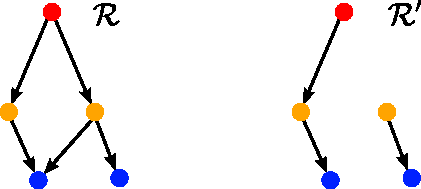
\includegraphics[height=3cm]{sections/major/fragments.pdf}
    \caption{Fragments \nick{Split into subfigures}
    }
    \label{fig:fragments}
\end{figure}

Any monotone is a trivial example of a resource fragment in the sense of the following~\cref{thm:monofrag}.
\begin{proposition}\label{thm:monofrag}
	Any monotone $\cal{M}$ of a resource theory $\R$ is a resource projection that maps the set of free states to $0$ and the pre-order $\prec_\R$ to a total order.
\end{proposition}
\begin{proof}
	Trivial.
\end{proof}
Mapping free states to real numbers and free operations to simple addition, the two conditions in the definition are equivalent to monotonicity and additivity respectively.
The ``free state'' for real numbers is 0 and all free states of the resource theory are mapped onto it.

The most general magic theory, the theory of Wigner negativity \nick{or positivity?}, can be expressed as $\R = (\F, \O)$ with
\begin{align}
    \F &= \{ \rho: \W[\bmz]{\rho} \geq 0\}\ \text{and} \\
    \O &= \{ \E: \W[\bmy|\bmx]{\E} \geq 0\}
\end{align}
for all points $\bmx, \bmy, \bmz \in \pd$.
Therefore, any free state $\sigma$ corresponds to a $d^2$-dimensional probability distribution $\W{\sigma}$ and any free operation $\E: \cal{B}(\hd) \mapsto \cal{B}(\hd)$ corresponds to a $d^2 \times d^2$ stochastic matrix (or conditional probability distribution) $\W{\E}$.
Note that these mappings are one-to-one due to the orthogonality of the phase-point operators as an operator basis.

Our goal is to give insight into magic state transformations.
We first break up the theory into fragments that allow for the incorporation of $\bmd$-majorization in its framework.
\begin{definition}[\textbf{$\boldsymbol\sigma$-fragment}]\label{def:sigmafrag}
    A subtheory $\R'$ of the Wigner negativity theory $\R = (\F, \O)$ is called a \emph{$\sigma$-fragment} iff $\R' = (\F, \O_\sigma)$, where the free operations are restricted to the ones that preserve $\sigma$,
    \begin{equation}
        \O_\sigma \coloneqq \{ \E \in \O: \E(\sigma) = \sigma \}.
    \end{equation}
\end{definition}

State $\sigma$ is thus a fixed point of all operations in $\O_\sigma$ and we provide the following theorem which characterises the $\sigma$-fragments as well as how they make up the whole set of free operations. \nick{move below}

\subsection{Majorization}\label{sec:major}

Majorization is a fundamental tool that has recently found many applications in quantum information theory \nick{CITE}.
It describes the \nick{disorder / non-uniformity} of vectors via stochastic transformations that are possible between them.

In order to discuss such stochastic transformations, we first denote by $\stoch$ the set of $(d \times d)$ stochastic matrices that preserve vector $\bmg$.
Specifically, any $S \in \stoch$ satisfies:
\begin{enumerate}
    \item $S_{ij} \geq 0$ for all $i, j \in \zd$;
    \item $\sum\limits_{j=1}^n S_{ij} = 1$ for all $i \in \zd$;
    \item $S\bmg = \bmg$.
\end{enumerate}
It forms a group under matrix multiplication because it contains the identity and $S^{-1} \in \stoch$ for any $S \in \stoch$.

We can motivate majorization very well for our purposes via its application on quantum thermodynamics in the absence of coherence.
At any given temperature $\beta$, the thermal state $\gamma_\beta$ is intuitively the most ordered state. 
Thermal operations are defined as operations that cannot extract energy from the Gibbs state, $\E(\gamma_\beta) = \gamma_\beta$.
Convertibility between states via thermal operations is equivalent to a stochasticity condition on the energy level populations of the states \nick{CITE}.
Roughly, the statement is that there exists a thermal operation $\E$ such that $\tau = \E(\rho)$ if and only if there exists a a matrix $S \in \stoch[\bmg]$ such that $\bm{q} = S\bm{p}$, where $\bm{q}, \bm{p}$ and $\bmg$ and the energy level population vectors of $\tau, \rho, \gamma_\beta$ respectively. \nick{expand or remove}

We can define majorization based on this definition.
\begin{definition}\label{def:dmajor}
    Given $\bmx, \bmy, \bmg \in \reals^d$, such that the components of $\bmg$ are positive, $\bmy$ is said to $\bmg$-majorize $\bmx$, iff there exists a matrix $S \in \stoch$ such that $\bmx = S\bmy$.
    
    We denote this partial order by $\bmx \prec_{\bmg} \bmy$.
\end{definition}
If $\bmg = \frac{1}{d}\bm{1}$, the $d$-dimensional uniform distribution, then $\stoch$ is the set of bistochastic matrices and we retrieve the familiar notion of majorization in entanglement theory. \nick{CITE}

A visual representation of $\bmg$-majorization is provided by the Lorenz curve of a vector $\bmz \in \reals^d$.
Let the vector $\bmz^\downarrow$ denote $\bmz$, but with its components arranged in non-increasing order.
\begin{definition}
    Let $\bmz \in \reals^n$.
    Let $\bmg \in \reals^d$ be a vector with positive components, $\pi$ a permutation mapping $(z_i/g_i) \mapsto (z_i/g_i)^\downarrow$ for all $i=1,\dots,d$ and $D = \sum_{i=1}^d g_i$.
    The Lorenz curve $L(\bmz|\bmg)$ of vector $\bmz$ is the piecewise linear curve obtained by joining the points 
\begin{equation}\label{eq:lorenz}
    \left\{ L_k(\bmz|\bmg) \coloneqq \left( \frac{1}{D}\sum_{i=1}^k g_{\pi(i)}, \sum_{i=1}^k z_{\pi(i)} \right) \in \mathbb{R}^2: k = 1,\dots,d \right\}.
\end{equation}
\end{definition}
\emph{Remark 1.} The origin $L_0(\bmz|\bmg) \coloneqq (0,0)$ is usually included in the curve.

\emph{Remark 2.} The first components of $L_k(\bmz|\bmg)$ are rescaled by $D$ so that comparison of curves with unequal dimensions is possible.
In fact, the Lorenz curves $L(\bmz|\bmg)$ and $L(\bmz \otimes \bmg|\bmg \otimes \bmg)$, where $\otimes$ denotes the Kronecker product, are identical.

\emph{Remark 3.} Lorenz curves are always concave.

\emph{Remark 4.} If $L_d(\bmz|\bmg) = 1$ and for all $k$, $L_k(\bmz|\bmg) \leq 1$, then $\bmz$ is a probability distribution.
Lorenz curves of quasi-probability distributions in principle reach above 1.

An example of comparison between different Lorenz curves is illustrated in~\cref{fig:lctoy}.
\begin{figure}
    \centering
    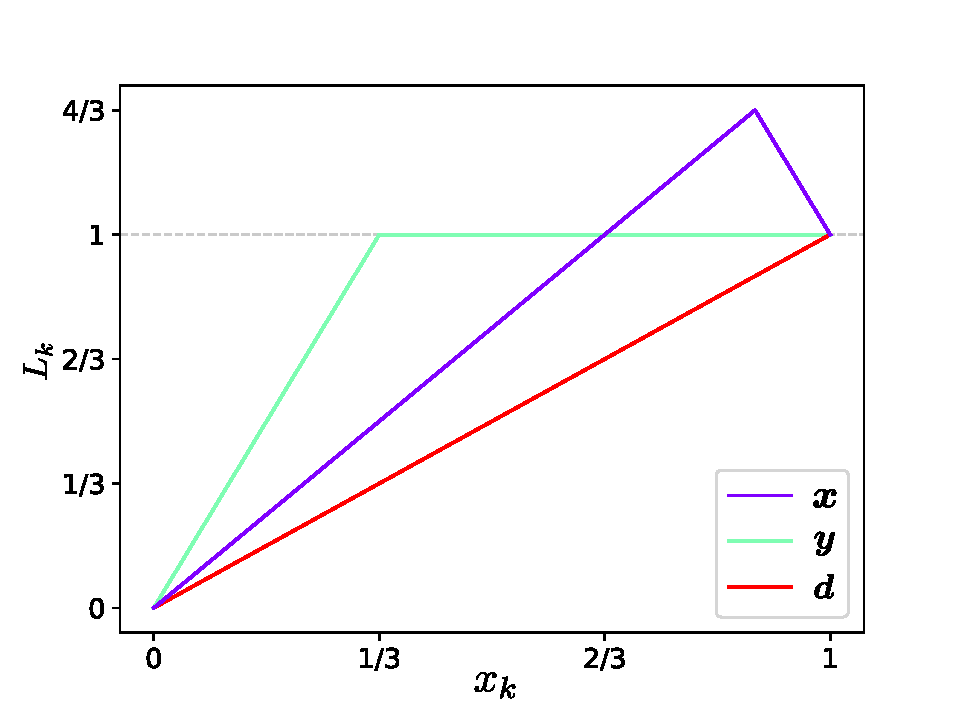
\includegraphics[height=5cm]{sections/major/lctoy.pdf}
    \caption{Example of different Lorenz curves for quasi-probability vectors under $\bmg$-majorization.
    Vectors $\bmy$ and $\bmg$ are simply probability distributions.
    The curve corresponding to vector $\bmg$ is always the straight line connecting $(0,0)$ and $(1,1)$, so that any other Lorenz curve lies above it, for example $\bmx \prec_{\bmg} \bmg$.
    Curves $L_k(\bmx|\bmg)$ and $L_k(\bmy|\bmg)$ intersect, so neither $\bmx \prec_{\bmg} \bmy$ nor $\bmy \prec_{\bmg} \bmx$.
    }
    \label{fig:lctoy}
\end{figure}

We now present the important majorization result needed in our analysis of magic.
\begin{theorem}\label{thm:dmajor}
Given $\bmx, \bmy, \bmg \in \reals^d$, such that the components of $\bmg$ are positive, the following statements are equivalent:
 \begin{enumerate}%[label=\enlabel{TM}{\arabic*}]
	\item\label{en:tm1} $\bmx \prec_{\bmg} \bmy$;
	\item\label{en:tm5} $L_k(\bmx|\bmg) \leq L_k(\bmy|\bmg)$ for all $k=1,2,\dots, d-1$ and $L_d(\bmx|\bmg) = L_d(\bmy|\bmg)$.
 \end{enumerate}
\end{theorem}
A restatement of the theorem including more equivalent conditions, along with a proof is provided in the \nick{appendix}.

\subsection{Magic fragments}\label{sec:magfrag}

\begin{theorem}\label{thm:frag}
    In the resource theory of Wigner negativity $\R = (\O, \F)$, the following statements hold:
    \begin{enumerate}
        \item The $\sigma$-fragment $\O_\sigma$ is equal to the set of all $\cptp$ operations with stochastic Wigner distributions that leave $\W{\sigma}$ invariant. \nick{Assuming maximal resource theory}
        \item Every free operation leaves at least one free state invariant such that $\O = \bigcup\limits_{\sigma \in \F} \O_\sigma$.
        \item If a free operation leaves two states invariant, then it also leaves every mixture of them invariant, $\O_{\sigma} \cap \O_{\sigma'} \subseteq \O_{p\sigma + (1-p)\sigma'}$ for all $p \in [0,1]$.
    \end{enumerate}
\end{theorem}
\begin{proof}
    \begin{enumerate}
    \item Let $\O_\sigma' \coloneqq \{ \E \in \cptp: \W{\E} \in \stochw \}$ be the described set of operations.
    
    Suppose $\E$ is in $\O_\sigma$, then $\E \in \cptp$ and $\W{\E} \in \stochw$ due to property~\ref{en:wo4} of~\cref{thm:wchannel}, hence $\O_\sigma \subseteq \O_\sigma'$.
    
    Conversely, suppose $\E \in \cptp$ with $\W{\E} \in \stochw$. 
    Then, $\W[\bmy|\bmx]{\E} \geq 0$ for all $\bmx, \bmy$, hence $\E \in \O$.
    Furthermore, $\W{\E} \W{\sigma} = \W{\sigma}$ implies $\E(\sigma) = \sigma$ using~\cref{eq:woperation} defined for any $\cptp$ operation $\E$.
    Hence, $\O_\sigma' \subseteq \O_\sigma$.
    
    \item Suppose $\E$ is in $\O_\sigma$, then it is also in $\O$, hence $\bigcup\limits_{\sigma \in \F} \O_\sigma \subseteq \O$.
    
    Conversely, suppose $\E$ is in $\O$. 
    The free states are mapped one-to-one to a subset $\cal{S}$ of the $(d^2 - 1)$-dimensional probability simplex.
    $\cal{S}$ is convex, since any combination of free states is also free and the Wigner distribution is linear.
    Therefore, $\cal{S}$ is convex and compact as a convex subset of the bounded compact probability simplex. \nick{Need to prove that $\cal{S}$ is closed.}
    Then, $\W{\E}{}$ is a stochastic, thus continuous, mapping from $\cal{S}$ to itself and Brouwer's fixed point theorem \nick{CITE} implies that there exists a probability distribution $g_{\bmz}, \bmz \in \pd$ that is preserved by $\W{\E}{}$.
    This corresponds one-to-one to a state $\sigma \coloneqq \sum_{\bmz \in \pd} g_{\bmz} A_{\bmz}$ and so $\O \subseteq \bigcup\limits_{\sigma \in \F} \O_\sigma$.
    
    \item Let $\E \in \O_{\sigma} \cap \O_{\sigma'}$.
    Then $\E \in \cptp$ and corresponds to stochastic Wigner distribution $\W{\E}$ such that $\W{\E} \W{\sigma} = \W{\sigma}$ and $\W{\E} \W{\sigma'} = \W{\sigma'}$.
    Then, $\W{\E} \W{p\sigma + (1-p)\sigma'} = \W{p\sigma + (1-p)\sigma'}$ for any $p \in [0,1]$ due to the additive property~\ref{en:w4} of the Wigner distribution, implying that state $p\sigma + (1-p)\sigma'$ is also left invariant by $\E$.
    \end{enumerate}
\end{proof}

The structure of the $\sigma$-fragment $(\F, \O_\sigma)$ for any $d$-dimensional $\sigma$ in $\F$ admits the pre-order of $\bmg$-majorization with $\bmg = \W{\sigma}$, a $d^2$-dimensional probability vector. 
If any component of $\W{\sigma}$ is zero, then we can always add some $\epsilon$ amount of unital noise by mixing $\sigma$ with the maximally mixed state $\frac{1}{d}\id$. 
This ensures that all components are strictly positive and $\bmd$-majorization can be used.

\begin{proposition}
    A state conversion $\rho \xrightarrow{\E \in \O} \tau$ is possible only if there exists a free state $\sigma$ such that for \nick{an infinitesimal $\epsilon$}, $\W{\tau} \prec_{\W{\sigma'}} \W{\rho}$, where $\sigma' = (1-\epsilon)\sigma + \epsilon \frac{1}{d}\id$.
\end{proposition}

\emph{Remark 1.} Note that free states $\F$ map onto a \emph{strict subset} of the set of probability distributions.
As a counterexample, consider the 9-dimensional probability distribution with non-zero components $\left(\frac{1}{2}, \frac{1}{4}, \frac{1}{4} \right)$. 
It does not correspond to any qutrit Wigner distribution because the component with value $\frac{1}{2}$ does not satisfy the boundedness condition~\ref{en:w3} of~\cref{thm:wstate}.

\emph{Remark 2.} Similarly, any $\O_\sigma$ may be mapped onto a \emph{strict subset} of the set $\stochw$ of stochastic matrices that preserve $\W{\sigma}{}$.

As an example, consider the permutation matrix
\begin{equation}
    \Pi_X = \begin{psmallmatrix}
        0 & 1 & 0 & 0 & 0 \\
        0 & 0 & 0 & 0 & 1 \\
        0 & 0 & 0 & 1 & 0 \\
        1 & 0 & 0 & 0 & 0 \\
        0 & 0 & 1 & 0 & 0
    \end{psmallmatrix} \otimes \begin{psmallmatrix}
        0 & 0 & 1 & 0 & 0 \\
        0 & 0 & 0 & 0 & 1 \\
        0 & 0 & 0 & 1 & 0 \\
        1 & 0 & 0 & 0 & 0 \\
        0 & 1 & 0 & 0 & 0    
    \end{psmallmatrix} \in \stochw,\ d=5.
\end{equation}
It preserves the uniform distribution $\W{\frac{1}{5}\id}{}$, but it does not correspond to any completely positive operation and therefore to any $\E \in \O$, due to~\cref{thm:frag}.

\emph{Remark 3.} No $\sigma$-fragment is empty.
In fact, an example of a stabilizer operation $\E \in \so \cap \O_\sigma$, for any $\sigma$-fragment, is the completely depolarising \nick{replacement} map
\begin{align}
    \E(\rho) &= \sigma \tr[\rho],\ \text{with} \\
    \W[\bmy|\bmx]{\E} &= \W[\bmy]{\sigma} \tr[\rho],
\end{align}
which can be thought as a sequence of tracing out state $\rho$ and preparing the stabilizer $\sigma$.

The zoo of all the operation classes is summarised in ~\cref{fig:zoo}.
Completely positive-Wigner-preserving operations ($\cpwp$) form the largest operation class in the literature.
Therefore, $\sigma$-fragments cover this theory of magic exactly and any magic subtheory is contained within this cover.
For example, the stabilizer-preserving ($\spo$)~\cite{cit:ahmadi} and completely stabilizer-preserving ($\cspo$)~\cite{cit:seddon} operation subclasses follow the hierarchy $\so \subset \cspo \subset \spo \subset \cpwp$ and therefore are described by our $\sigma$-fragments.

\begin{figure}
    \centering
        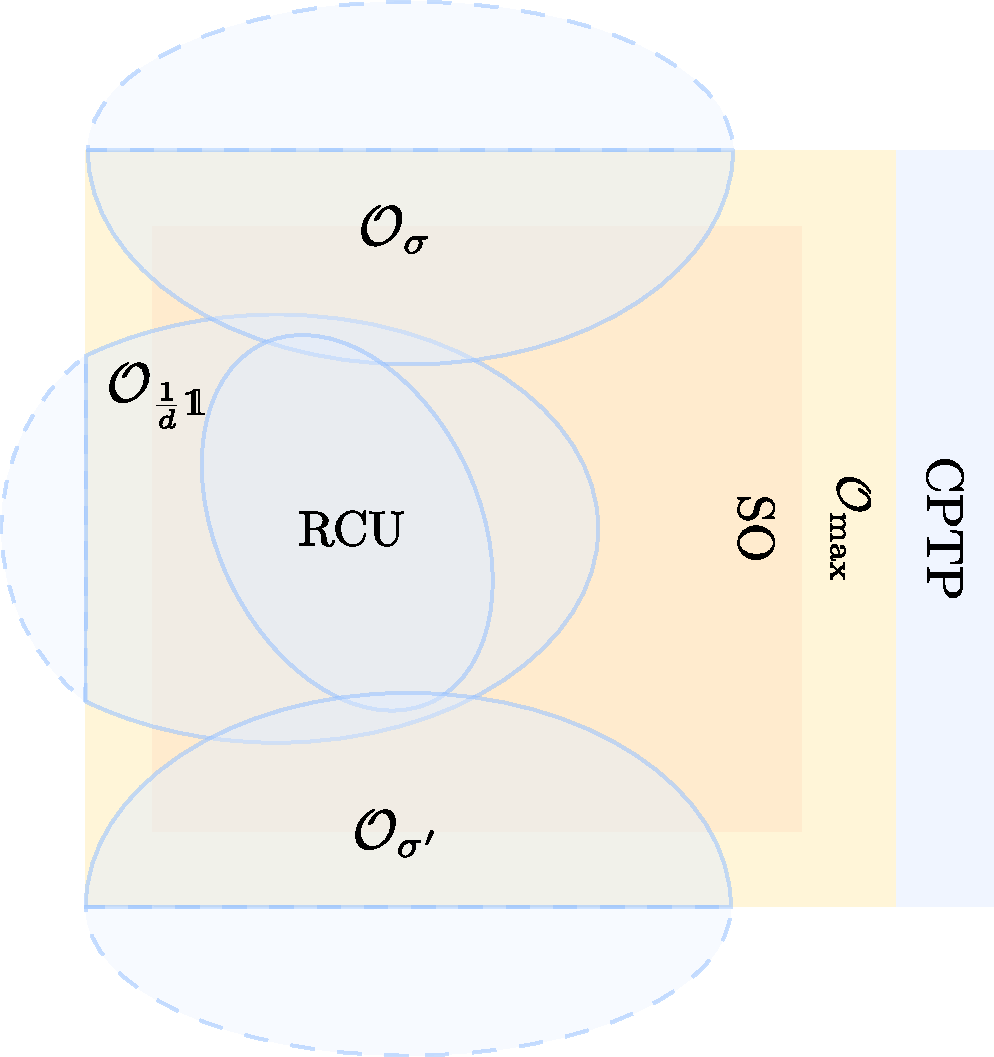
\includegraphics[scale=0.5]{sections/major/operations.pdf}
    \caption{Zoo of allowed operations for magic resource theories.
    Established theories involve operations within the yellow regions, following the hierarchy $\so \subset \cspo \subset \spo \subset \cpwp$.
    We introduce fragments $\O_\sigma \subset \stochw,\ \sigma \in \F$ that cover $\cpwp$ with each one extending to a set of stochastic maps that allows for $\bmd$-majorization to be used.
    \nick{fragments are the intersections of blue and orange, not the whole bubble - technically $\stochw$ should be replaced by its operational pre-image.}
    }
    \label{fig:zoo}
\end{figure}